\begin{table*}[t!]
\small
  \centering
    \begin{tabular*}{\textwidth}{l|c|c|c|c|c@{}}
    \hline
    Segmentation                & Learning           & Type of          & PSB rand index (\# train. & L-PSB  accuracy (\# train.  & COSEG          \\
    method                      & type               & manual input     & shapes if applicable)     & shapes if applicable)       & accuracy       \\
    \hline
    \hline
    \cite{Kalogerakis:2010:LMS} & supervised         & labeled shapes   & 9.4\% (19) / 14.8\% (3)   & 95.3\% (19) / 89.2\% (3)    & 91.9\% (12) / 89.0\% (3) \\
    \hline
    \cite{Benhabiles:2011:LBE}  & supervised         & segmented shapes & 8.8\% (19) / 9.7\% (6)    & not applicable              & not applicable \\
    \hline
    \cite{Huang:2011:JSS}       & unsupervised       & none             & 10.1\%                    & not applicable              & not applicable \\
    \hline
    \cite{Sidi:2011:CS}         & unsupervised       & none             & unknown                   & unknown                     & 87.7\%         \\
    \hline
    \cite{van-Kaick:2011:PKC}   & supervised         & labeled shapes   & unknown                   & \~88.7\% (12), see caption   & unknown        \\
    \hline
    \cite{Hu:2012:CSS}          & unsupervised       & none             & unknown                   & 88.5\%                      & 91.4\%         \\
    \hline
    \cite{Lv:2012:SMS}          & semi-supervised    & labeled shapes   & unknown                   & 92.3\% (3)                  & unknown        \\
    \hline
%    \cite{Wang:2012:ACS}        & semi-supervised    & link constraints & unknown                   & unknown                     & `close to error-free' \\
%    \hline
    \cite{Wang:2013:PAS}        & supervised         & labeled images   & unknown                   & \~88.0\% (19), see caption   & unknown               \\
    \hline
    \cite{Kim:2013:lpt}         & semi-/unsupervised & box templates    & unknown                   & unknown                     & 92.7\% (semi-superv.) \\
    \hline
    \cite{Huang:2014:FMN}       & unsupervised       & none             & unknown                   & unknown                     & 90.1\%                \\
    \hline
    \cite{Xu:2014:TSS}          & supervised         & labeled shapes   & 10.0\%                    & 86.0\%                      & unknown               \\
    \hline
    \cite{Zhige:2014:SSL}       & supervised         & labeled shapes   & 10.2\% (19)               & 94.2 (19) / 88.6 (5)        & unknown               \\
    \hline
%    \cite{Yi:2016aa}       & semi-supervised         & labeled views and verifications   & unknown               & unknown        & 100\% human-verified               \\
%    \hline
    \end{tabular*}%
  \caption{\rev{Performance of data-driven methods for segmentation in the Princeton Segmentation Benchmark (PSB) and COSEG datasets.
		   Left to right: segmentation method, learning type depending on the nature of data required as input to the method, type of manual input if such required, segmentation performance expressed by the rand index metric \protect\cite{Chen:2009:BMS}, labeling accuracy \protect\cite{Kalogerakis:2010:LMS} based on the PSB and COSEG datasets. 	
  		   We report the rand index segmentation error metric averaged over all classes of the PSB benchmark.
  		   The labeling accuracy is averaged over the Labeled PSB (L-PSB) benchmark excluding the ``Bust'', ``Mech'', and ``Bearing'' classes. The reason is that there are no clear semantic correspondences between parts in these classes, or the ground-truth segmentations do not sufficiently capture semantic parts in their shapes.
  		   We report the labeling accuracy averaged over the categories of the COSEG dataset used in \protect\cite{Sidi:2011:CS}. The COSEG classes ``iron'', ``large chairs'', ``large vases'', ``tele-aliens'' were added later and are excluded here since most papers frequently do not report performance in those.
  		   We note that van Kaick et al.~\protect\cite{van-Kaick:2011:PKC} reported the labeling accuracy in ten of the L-PSB classes, while Wang et al.~\protect\cite{Wang:2013:PAS}  reported the labeling accuracy in seven of the L-PSB classes.
  		   The method by Kim et al.~\protect\cite{Kim:2013:lpt} can run in either semi-supervised or unsupervised mode. In unsupervised mode, the corresponding labeling accuracy is 89.9\% in the COSEG dataset on average.
  		   }}
  \label{tab:segmentation_performance}%
\end{table*}


\section{Shape segmentation}
\label{sec:segmentation}

The goal of data-driven shape segmentation is to partition the shapes of an input collection into parts, and also estimate part correspondences across these shapes. We organize the literature on shape segmentation into the following three categories: supervised segmentation, unsupervised segmentation, and semi-supervised segmentation following the main classification discussed in Section \ref{sec:overview}. \rev{Table \ref{tab:segmentation_performance} summarizes representative techniques and reports their segmentation and part labeling performance based on established benchmarks. Table \ref{tab:segmentation_running_times} reports characteristic running times for the same techniques.}

%For example, a data-driven segmentation algorithm can segment the shapes of an input collection of chairs into parts, such as legs, back, and seat.

%There is no unique way to segment a shape:
%the user can provide a set of exemplar shape segmentations, desired part correspondences, or parameters to control the type and level of detail for segmentation. Alternatively, shapes can be consistently segmented at various levels of detail, and the segments can be organized hierarchically.

\begin{figure}[t]
\centering
    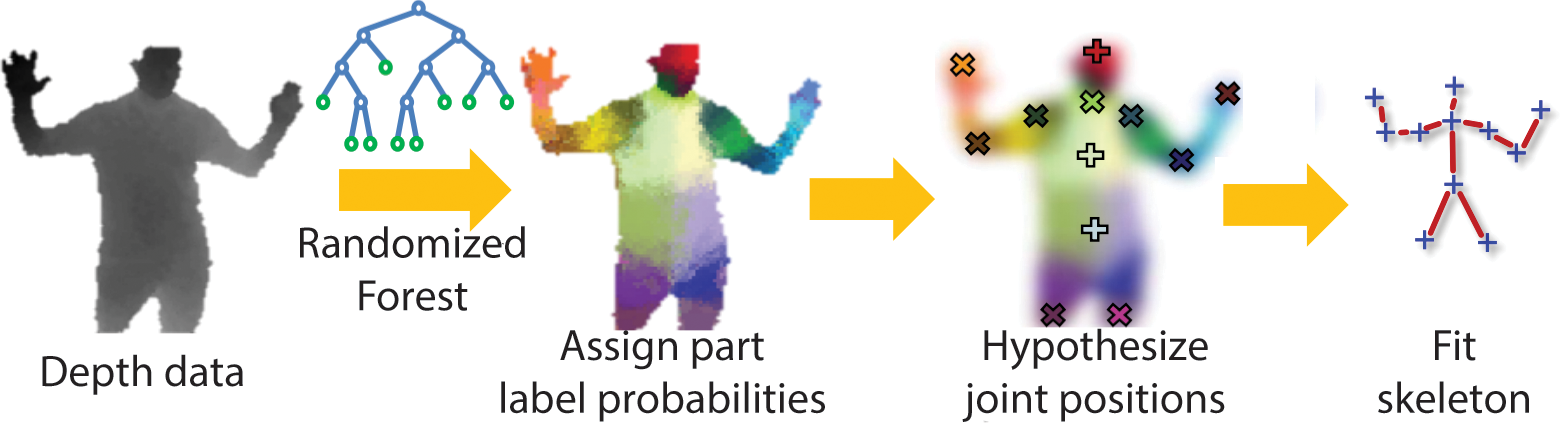
\includegraphics[width=1.0\columnwidth]{fig/img/kinect}
    %\vspace{-0.4cm}
    \caption{
    A random forest classifier applied on depth data representing a human body shape (image from \protect\cite{Fossati:2013:CDC}) }
    \label{fig:kinect}
\end{figure}



\subsection{Supervised shape segmentation}

\paragraph*{Classification techniques.} Supervised shape segmentation is frequently formulated as a classification problem. Given a training set of shapes containing points, faces or patches that are labeled according to a part category (see Figure \ref{fig:overview_seg}), the goal of a classifier is to identify which part category other points, faces, or patches from different shapes belong to. Supervised shape segmentation is executed in two steps: during the first step, the parameters of the classifier are learned from the training data. During the second step, the classifier is applied on new shapes. A simple linear classifier has the form:
\begin{equation}
c = f ( \sum\limits_j \theta_j \cdot x_j )
\end{equation}
where $x_j$ is a geometric feature of a point (face, or patch), such as the ones discussed in Section \ref{sec:overview}. The parameters $\theta_j$ serve as weights for each geometric feature. The function $f$ is non-linear and maps to a discrete value (label), which is a part category, or to probabilities per category. In general, choosing a good set of geometric features that help predicting part labels, and employing classifiers that can discriminate the input data points correctly are important design choices. There is no rule of thumb on which is the best classifier for a problem. This depends on the underlying distribution and characteristics of the input geometric features, their dimensionality, amount of labeled data, existence of noise in the labeled data or shapes, training and test time constraints - for a related discussion on how to choose a classifier for a problem, we refer the reader to \cite{Manning:2008:IIR}. Due to the large dimensionality and complexity of geometric feature spaces, non-linear classifiers are more commonly used. For example, to segment human bodies into parts and recognize poses, the Microsoft's Kinect uses a random forest classifier trained on synthetic depth images of humans of many shapes and sizes in highly varied poses sampled from a large motion capture database \cite{Shotton:2011:RLH} (Figure \ref{fig:kinect}).


\paragraph*{Structured models.} For computer graphics applications, it is important to segment shapes with accurate and smooth boundaries. For example, to help the user create a new shape by re-combining parts from other shapes \cite{Funkhouser:2004:MBE}, irregular and noisy segmentation boundaries can cause problems in the part attachment. From this aspect, using a classifier per point/face independently is usually not enough. Thus, it is more common to formulate the shape segmentation problem as an energy minimization problem that involves a unary term assessing the consistency of each point/face with each part label, as well as a pairwise term assessing the consistency of neighboring points/faces with pairs of labels. For example, pairs of points that have low curvature (i.e., are on flat surface) are more likely to have the same part label. This energy minimization formulation has been used in several single-shape and data-driven segmentations (unsupervised or supervised) \cite{Katz:2003:HMD,Anguelov:2005:DLM,Shapira:2010:CPA,Kalogerakis:2010:LMS}. In the case of supervised segmentation \cite{Kalogerakis:2010:LMS}, the energy can be written as:
\begin{equation}
E(\bc; \theta) = \sum_i E_{unary}(c_i; \bx_i, \theta_1) + \sum_{i,j} E_{pairwise}(c_i, c_j; \by_{ij}, \theta_2)
\label{eqn:CRFEnergy}
\end{equation}
where $\bc=\{c_i\}$ is a vector of random variables representing the part label per point (or face) $i$, $\bx_i$ is its geometric feature vector, $i,j$ are indices to points (or faces) that are considered neighbors, $\by_{ij}$ is a geometric feature vector representing dihedral angle, angle between normals, or other features, and $\theta=\{\theta_1,\theta_2\}$  are the energy parameters.  The important difference of supervised data-driven methods with previous single-shape segmentation methods is that the parameters $\theta$ are automatically learned from the training shapes to capture complex feature space patterns per part \cite{Anguelov:2005:DLM,Kalogerakis:2010:LMS}. We also note that the above energy of Equation \ref{eqn:CRFEnergy}, when written in an exponentiated form and normalized, can be treated as a probabilistic graphical model \cite{Koller:2009:PGM}, called Conditional Random Field \cite{Lafferty:2001:CRF} that represents the joint probability distribution over part labels conditioned on the input features:
\begin{equation}
P(\bc | \bx, \by, \theta)= \exp(-E(\bc;\theta))/ Z(\bx,\by,\theta)
\label{eqn:CRFConditional}
\end{equation}
where $Z(\bx,\by,\theta)$ is a normalization factor, also known as partition function. \rev{Minimizing the energy of Equation \ref{eqn:CRFEnergy}, or correspondingly finding the assignment $\bc$ that maximizes the above probability distribution is known as a Maximum A Posteriori inference problem that can be solved in various manners, such as graph cuts, belief propagation, variational or linear programming relaxation techniques \cite{Koller:2009:PGM}.}


The parameters $\theta$ can be jointly learned through maximum likelihood (ML) or maximum a posteriori (MAP) estimates \cite{Koller:2009:PGM}. However, due to high computational complexity of ML or MAP learning and the non-linearity of classifiers used in shape segmentation, it is common to train the parameters $\theta_1$ and $\theta_2$ of the model separately i.e., train the classifiers of the unary and pairwise term separately \cite{Sutton:2005:PTU}. The exact form of the unary and pairwise terms vary across supervised shape segmentation methods: the unary term can have the form of a log-linear model \cite{Anguelov:2005:DLM}, cascade of JointBoost classifiers \cite{Kalogerakis:2010:LMS}, Gentleboost \cite{van-Kaick:2011:PKC}, or feedforward neural networks \cite{Zhige:2014:SSL}. The pairwise term can have the form of a learned log-linear model \cite{Anguelov:2005:DLM}, label-dependent GentleBoost classifier \cite{Kalogerakis:2010:LMS}, or a smoothness term based on dihedral angles and edge length tuned by experimentation \cite{Shapira:2010:CPA,van-Kaick:2011:PKC,Zhige:2014:SSL}. Again the form of the unary and pairwise terms depend on the amount of training data, dimensionality and underlying distribution of geometric features used, and computational cost.


\begin{table*}[t!]
\small
  \centering
    \begin{tabular}{l|c|c|c}
    \hline
    Segmentation                & Reported                     &  Dataset size for       & Reported \\
    method                      & running times                &  reported running times & processor \\
    \hline
    \hline
    \cite{Kalogerakis:2010:LMS} & 8h train. / 5 min test.      &  6 train. shapes / 1 test shape     & Intel Xeon E5355 2.66GHz \\
    \hline
    \cite{Benhabiles:2011:LBE}  & 10 min train. / 1 min test.  &  unknown for train. / 1 test shape  & Intel Core 2 Duo 2.99GHz \\
    \hline
    \cite{Huang:2011:JSS}       & 32h                          &  380 shapes                         & unknown, 2.4 GHz \\
    \hline
    \cite{Sidi:2011:CS}         & 10 min                       &  30 shapes                          & AMD Opteron 2.4GHz \\
    \hline
    \cite{van-Kaick:2011:PKC}   & 10h train. / few min test.   &  20-30 train. shapes / 1 test shape & AMD Opteron 1GHz  \\
    \hline
    \cite{Hu:2012:CSS}          & 8 min (excl. feat. extr.)    &  20 shapes                          & Intel dual-core 2.93GHz  \\
    \hline
    \cite{Lv:2012:SMS}          & 7h train. / few min test.    &  20 shapes                          & Intel I7 2600 3.4GHz \\
    \hline
%    \cite{Wang:2012:ACS}        & 7 min user interaction       &  28 shapes                          & unknown \\
%    \hline
    \cite{Wang:2013:PAS}        & 1.5 min (no train. step)     &  1 test shape                       & unknown \\
    \hline
    \cite{Kim:2013:lpt}         & 11h                          &  7442 shapes                        & unknown \\
    \hline
    \cite{Huang:2014:FMN}       & 33h                          &  8401 shapes                        & unknown, 3.2GHZ \\
    \hline
    \cite{Xu:2014:TSS}          & 30 sec (no train. step)      &  1 test shape                       & Intel I5 CPU \\
    \hline
    \cite{Zhige:2014:SSL}       & 15 sec train. (excl. feat. extr.) &  6 train. shapes                & Intel Quad-Core 3.2 GHz \\
    \hline
    \end{tabular}%
  \caption{\rev{Running times reported for the data-driven segmentation methods of Table \ref{tab:segmentation_performance}. We note that running times are reported in different dataset sizes and processors in the referenced papers, while it is frequently not specified whether the execution uses one or multiple threads or whether the running times include all the algorithm steps, such as super-face or feature extraction.
           Exact processor information is also frequently not provided. Thus, the reported running times of this table are only indicative and should not serve as a basis for a fair comparison.}}
  \label{tab:segmentation_running_times}%
\end{table*}



\paragraph*{Joint labeling.} Instead of applying the learned probabilistic model to a single shape, an alternative approach is to find correspondences between faces of pairs of shapes, and incorporate a third ``inter-shape'' term in the energy of Equation \ref{eqn:CRFEnergy} \cite{van-Kaick:2011:PKC}. The ``inter-shape'' term favors pairs of corresponding faces on different shapes to have the same label. As a result, the energy can be minimized jointly over a set of shapes to take into account any additional correspondences.



\paragraph*{Boundary learning.} Instead of applying a classifier per mesh point, face or patch to predict a part label, a different approach is to predict the probability that a polygon mesh edge is a segmentation boundary \cite{Benhabiles:2011:LBE}. The problem can be formulated as a binary classifier (e.g., Adaboost) that is trained from human segmentation boundaries. The input to the classifier are geometric features of edges, such as dihedral angles, curvature, and shape diameter. The output is a probability for an edge to be a segmentation boundary. Since the predicted probabilities over the mesh do not correspond to closed smooth boundaries, a thinning and an active contour model \cite{Kass:1988:SAC} are used in post-processing to produce the final segmentations.
%The output is not a labeled segmentation as in previous techniques, but a set of candidate segmentation boundaries. The method has currently the best performance in segmentation according to the Rand Index criterion in the PSB benchmark \cite{Chen:2009:BMS}.

\paragraph*{Transductive segmentation.} Another way to formulate the shape segmentation problem is to group patches on a mesh such that the segment similarity is maximized between the resulting segments and the provided segments in the training database. The segment similarity can be measured as the reconstruction cost of the resulting segment from the training ones. The grouping of patches can be solved as an integer programming problem \cite{Xu:2014:TSS}.

\paragraph*{Shape segmentation from labeled images.} \rev{Instead of using labeled training shapes for supervised shape segmentation, an alternative source of training data can come in the form of segmented and labeled images, as demonstrated by Wang et al. \cite{Wang:2013:PAS}. Given an input 3D shape, this method first renders 2D binary images of it from different viewpoints. Each binary image is used to retrieve multiple segmented and labeled training images from an input database based on a bi-class Hausdorff distance measure. Each retrieved image is used to perform label transfer to the 2D shape projections. All labeled projections are then back-projected onto the input 3D model to compute a labeling probability map. The energy function for segmentation is formulated by using this probability map in the unary term expressed per face or point, while dihedral angles and Euclidean distances are used in the pairwise term.}


\subsection{Semi-supervised shape segmentation}

\paragraph*{Entropy regularization.} The parameters $\theta$ of \rev{Equation \ref{eqn:CRFEnergy}} can be learned not only from the training labeled shapes, but also from the unlabeled shapes \cite{Lv:2012:SMS}. The idea is that learning should maximize the likelihood function of the parameters over the labeled shapes, and also minimize the entropy (uncertainty) of the classifier over the unlabeled shapes (or correspondingly maximize the negative entropy). The idea is that minimizing the entropy over unlabeled shapes encourages the algorithm to find putative labelings for the unlabeled data \cite{Jiao:2006:SCR}. However, it is generally hard to strike a balance between the likelihood and entropy terms.

\paragraph*{Metric embedding and active learning.} A more general formulation for semi-supervised segmentation was presented in \cite{Wang:2012:ACS}.
%(Figure \ref{fig:active_coanalysis}).
Starting from a set of shapes that are co-segmented in an unsupervised manner \cite{Sidi:2011:CS}, the user interactively adds two types of constraints: ``must-link'' constraints, which specify that two patches (super-faces) should belong to the same cluster, and ``cannot-link'' constraints which specify that two patches  must be in different clusters. These constraints are used to perform constrained clustering in an embedded feature space of super-faces coming from all the shapes of the input dataset. The key idea is to transform the original feature space, such that super-faces with ``must-link'' constraints come closer together to form a cluster in the embedded feature space, while super-faces with ``cannot-link'' constraints move away from each other. To minimize the effort required from the user, the method suggests to the user pairs of points in feature space that when constrained are likely to improve the co-segmentation.  The suggestions involve points that are far from their cluster centers, and have a low confidence of belonging to their clusters. \revnew{Yi et al.~\cite{Yi:2016aa} propose a method for achieving accurate segmentation of a dataset. Their method balances between manual mesh labeling, automatic propagation of these annotations, and verification of manual and automatic annotations. Their optimization explicitly minimizes the expected human work time. }

\paragraph*{Template fitting.} \rev{A different form of partial supervision can come in the form of part-based templates. Kim et al.'s method \cite{Kim:2013:lpt} allows users to specify or refine a few templates made out of boxes representing expected parts in an input database. The boxes iteratively fit to the shapes of a collection through simultaneous alignment, surface segmentation and point-to-point correspondences estimated between each template and each input shape. Alternatively, the templates can be inferred automatically from the shapes of the input collection without human supervision based on single shape segmentation heuristics. Optionally, the user can refine and improve these estimated templates. From this aspect, Kim et al.'s method can run in either a semi-supervised or unsupervised method. It was also the first method to handle segmentation and correspondences in collections with size on the order of thousands of shapes.}


\subsection{Unsupervised segmentation}

Unsupervised data-driven shape segmentation techniques fall into two categories: clustering based techniques and matching based techniques. In the following, we highlight the key idea of each type of approach.
% and review representative works.

\para{Clustering} based techniques are adapted from supervised techniques. They compute feature descriptors on points or faces. Clustering is performed over all points/faces over all shapes. Each resulting cluster indicates a consistent segment across the input shapes. The promise of the clustering based approach is that when the number of shapes becomes large, the sampling density in the clustering space becomes dense enough, so that certain statistical assumptions are satisfied, e.g., diffusion distances between points from different clusters is significantly larger than those between points within each cluster. \rev{When these assumptions are satisfied, clustering based approaches may produce results that are comparable to supervised techniques (c.f.~\cite{Hu:2012:CSS}) . In~\cite{Sidi:2011:CS}, the authors utilize spectral clustering to perform clustering. In~\cite{Hu:2012:CSS}, the authors employ subspace clustering, a more advanced clustering method, to obtain improved results.}

Clustering methods can also be applied to shape parts. In~\cite{Xu:2010:SCS}, the authors perform co-analysis over a set of shapes via factoring out the part scale variation by grouping the shapes into different styles, where style is defined by the anisotropic part scales of the shapes. In~\cite{van-Kaick:2013:CHA}, the authors introduce unsupervised co-hierarchical analysis of a set of shapes. They propose a novel cluster-and-select scheme for selecting representative part hierarchies for all shapes and grouping the shapes according to the hierarchies. The method can be used to compute consistent hierarchical segmentations for the input set.

\begin{figure}[t!]
\centering
    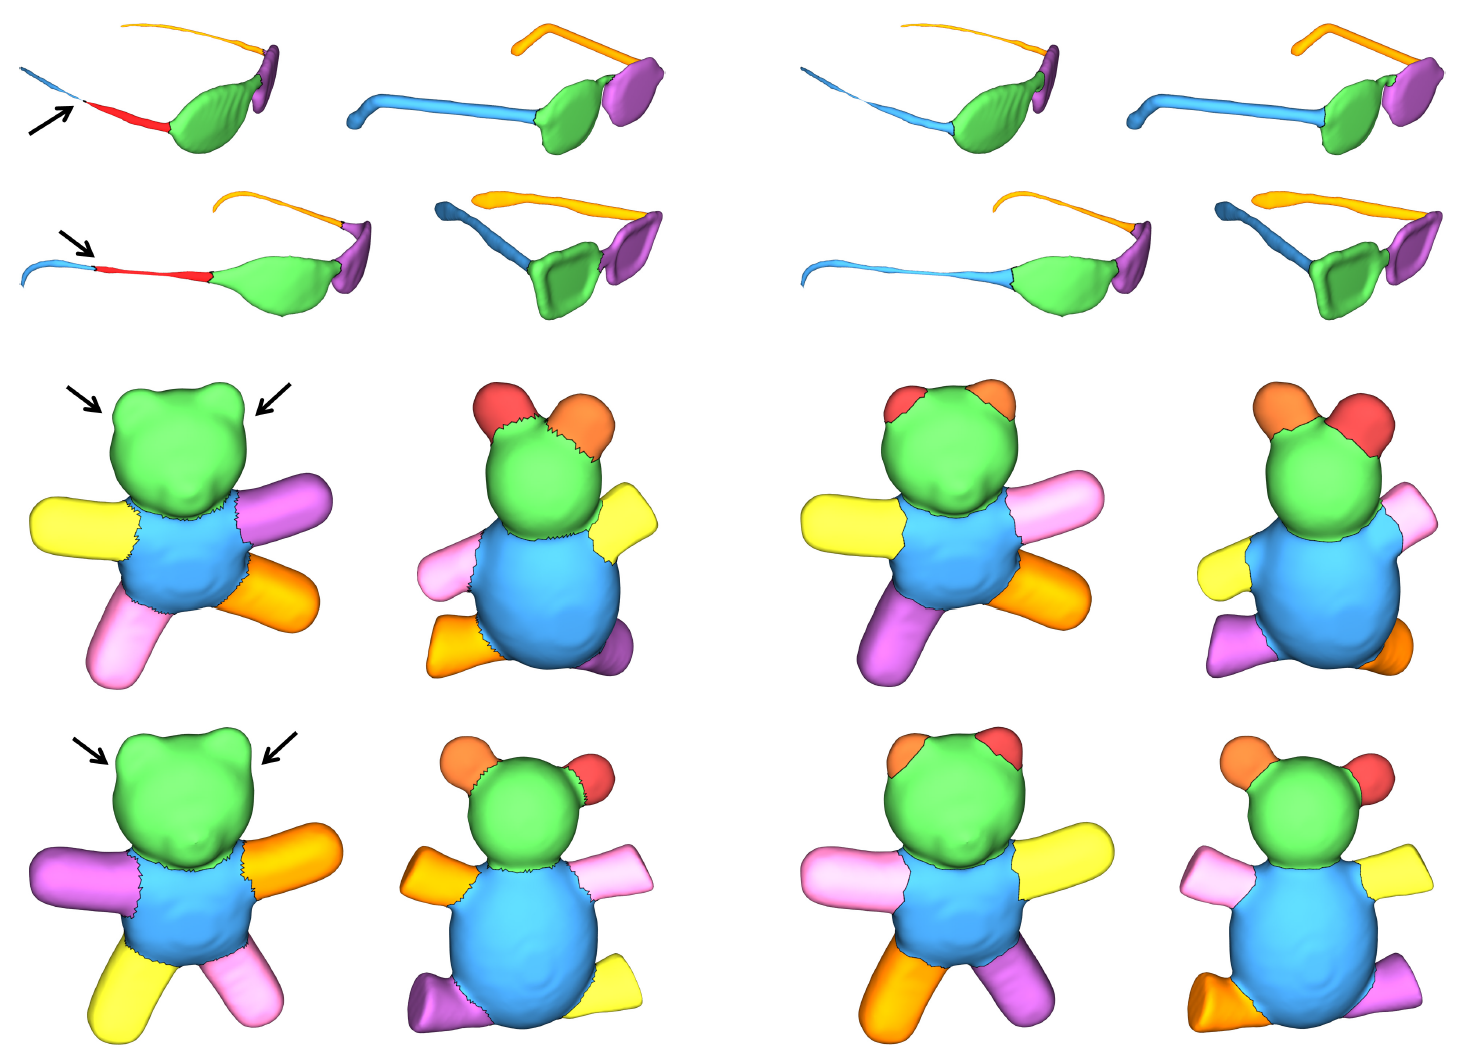
\includegraphics[width=1.0\columnwidth]{fig/img/huang_siga11_jss.png}
    %\vspace{-0.5cm}
    \caption{Comparison of single-shape segmentation (left) and joint shape segmentation (right) on models from the PSB benchmark~\cite{Chen:2009:BMS}. Each segmentation on the left was produced by the top-performing algorithm in the benchmark for that shape. The segmentations on the right were produced
by~\cite{Huang:2011:JSS}, which jointly optimized segmentations and correspondences across the entire dataset.}
    \label{fig:huang_siga11_jss}
\end{figure}



\para{Matching} based methods~\cite{Golovinskiy:2009:CS,Huang:2011:JSS,Wang:2013:FMap,Huang:2014:FMN} build maps across shapes and utilize these maps to achieve consistency of segmentations. As shown in Figure~\ref{fig:huang_siga11_jss}, this strategy allows us to identify meaningful parts despite the lack of strong geometric cues on a particular shape. Likewise, the approach is able to identify coherent single parts even when the geometry of the individual shape suggests the presence of multiple segments. A challenge here is to find a suitable shape representation so that maps across diverse shapes are well-defined. In~\cite{Huang:2011:JSS}, Huang et al. introduce an optimization strategy that jointly optimizes shape segmentations and maps between optimized segmentations. Since the maps are defined at the part-level, this technique is suitable for heterogeneous shape collections. Experimentally, it generates comparable results with supervised method~\cite{Kalogerakis:2010:LMS} on the Princeton segmentation benchmark.  Recently, Huang et al.\cite{Huang:2014:FMN} formulated the same idea under the framework of functional maps~\cite{Ovsjanikov:2012:FMF} and gain improved segmentation quality and computational efficiency.
